The brain of the Traffic Pi device. Center of the architectural design that sens and receives from the other component layers. Takes in the data acquired from vision, housed in the case, driven from the power layer, and communicates with the application to transmit the desired information for the user. The computer layer determines when to active and record its surroundings and process the data then stores it for further use from the application layer.

\subsection{Interface}
The central bus mechanism the connects to computer layer's surrounding layers.

\begin{figure}[h!]
	\centering
 	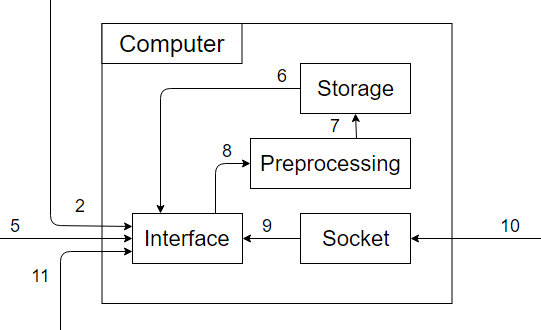
\includegraphics[width=0.60\textwidth]{images/computer_subsystem.png}
 \caption{Computer Interface subsystem diagram}
\end{figure}

\subsubsection{Assumptions}
Assume the interface is uninterrupted and successfully communicates with the other layers and power socket.

\subsubsection{Responsibilities}
Serves as the central hub for transmitting and receiving information from the vision, case, application layers and the power socket sub-layer. Electrical power from the socket will the cooling mechanism and the cameras, then from data collected from vision if a car is detected the computer interface will signal pre-process to take in data like footage (frames), distance, time stamps, and car ID assignment. Will transmit data to the case layer's cooling system to maintain proper temperate condition to avoid overheating given heat generated and environmental heat. Computer interface will once connected to a home computer and commanded to direct stored data for the user it will direct to the application layer's interface. Signals can be redirected back in case of malfunctions, errors, or corrupted data.

\subsubsection{Subsystem Interfaces}

\begin {table}[H]
\caption {Computer interfaces} 
\begin{center}
    \begin{tabular}{ | p{1cm} | p{6cm} | p{3cm} | p{3cm} |}
    \hline
    ID & Description & Inputs & Outputs \\ \hline
    \#2 & Directs power to cooling system and receive temperature data & \pbox{3cm}{Temp data} & \pbox{3cm}{Electric power (watts)}  \\ \hline
    \#5 & Directs power and receive camera data & \pbox{3cm}{Footage (frames) \\ Distance (meters) \\ Car ID} & \pbox{3cm}{Electric power (watts)}  \\ \hline
    \#6 & Storage data stream through Interface and towards the application layer or to continue with normal operations & \pbox{3cm}{N/A} & \pbox{3cm}{Footage (frames) \\ Distance (meters) \\ Car ID \\ Time stamp}  \\ \hline
    \#8 & Data from vision to go through pre-processing to be looked over and formatted for later use or called by user to be displayed on their local machine & \pbox{3cm}{N/A} & \pbox{3cm}{Footage (frames) \\ Distance (meters) \\ Car ID}  \\ \hline
    \#9 & Mechanical socket transmitting electrical power & \pbox{3cm}{Electric power (watts)} & \pbox{3cm}{N/A}  \\ \hline
    \#11 & The Traffic Pi connected with the user's home computer and communicates through the pre-installed program on their machine & \pbox{3cm}{Error Signal} & \pbox{3cm}{Footage (frames) \\ Distance (meters) \\ Car ID \\ Time stamp}  \\ \hline
    \end{tabular}
\end{center}
\end{table}

\subsection{Pre-process}
Takes in the data given from the interface layer and sets up the data format to be stored and later use in the application layer.

\begin{figure}[h!]
	\centering
 	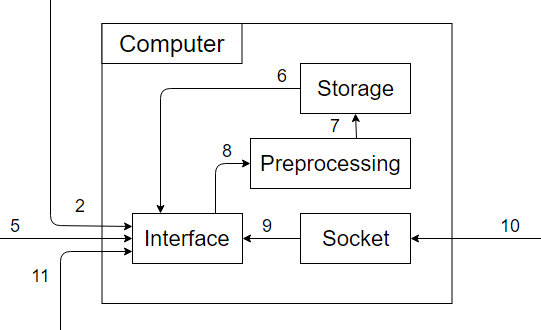
\includegraphics[width=0.60\textwidth]{images/computer_subsystem.png}
 \caption{Pre-process subsystem diagram}
\end{figure}

\subsubsection{Assumptions}
Assume the data collected and given is not corrupted nor illegal for the formatting.

\subsubsection{Responsibilities}
The pre-process sub-layer is responsible for formatting given data from the interface sub-layer from the vision layer. Data given would include footage (frames), distance, time stamps, and car ID assignment, then formats them to be stored in the storage for later processing in the application layer. The purpose of this is to not strain the computer layer's ability to capture the required variable data from passing cars by computing speed and streaming video data at the same time.

\subsubsection{Subsystem Interfaces}

\begin {table}[H]
\caption {Pre-process subsystem interfaces} 
\begin{center}
    \begin{tabular}{ | p{1cm} | p{6cm} | p{3cm} | p{3cm} |}
    \hline
    ID & Description & Inputs & Outputs \\ \hline
    \#7 & Post pre-processing to be stored or signalled by user to collect storage data & \pbox{3cm}{N/A} & \pbox{3cm}{Footage (frames) \\ Distance (meters) \\ Car ID \\ Time stamp}  \\ \hline
    \#8 & Data from vision to go through pre-processing to be looked over and formatted for later use or called by user to be displayed on their local machine & \pbox{3cm}{Footage (frames) \\ Distance (meters) \\ Car ID} & \pbox{3cm}{N/A}  \\ \hline
    \end{tabular}
\end{center}
\end{table}

\subsection{Storage}
The sub-layer tasked to simple store the data from pre-process and later access for future computational work.

\begin{figure}[h!]
	\centering
 	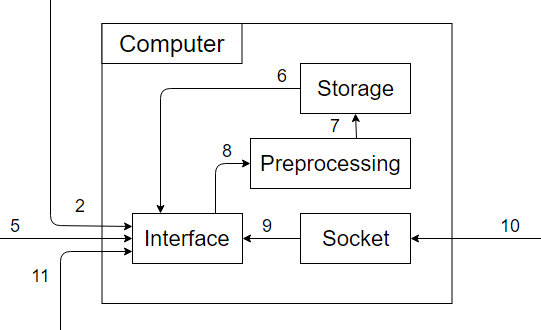
\includegraphics[width=0.60\textwidth]{images/computer_subsystem.png}
 \caption{Storage subsystem diagram}
\end{figure}

\subsubsection{Assumptions}
Assume the storage will be able to hold enough data for a mildly used road and will not fall under mechanical malfunctions.

\subsubsection{Responsibilities}
Storage is to hold formatted files from pre-process and returns the Traffic Pi to continue collecting data. Once the Traffic Pi is picked up and connected to the user's home computer then requested to take the formatted data to be calculated and viewed, the storage sub-system will send the data through computer layer's interface then onto the application layer. If the data was found to be corrupted the  application will request either a troubleshoot or another request of storage's data.

\subsubsection{Subsystem Interfaces}

\begin {table}[H]
\caption {Storage subsystem interfaces} 
\begin{center}
    \begin{tabular}{ | p{1cm} | p{6cm} | p{3cm} | p{3cm} |}
    \hline
    ID & Description & Inputs & Outputs \\ \hline
    \#6 & Continues devices normal operations unless signalled by the user to stream data into their local machine & \pbox{3cm}{Footage (frames) \\ Distance (meters) \\ Car ID \\ Time stamp} & \pbox{3cm}{N/A}  \\ \hline
    \#7 & Post pre-processing to be stored or signalled by user to collect storage data & \pbox{3cm}{Footage (frames) \\ Distance (meters) \\ Car ID \\ Time stamp} & \pbox{3cm}{N/A}  \\ \hline
    \end{tabular}
\end{center}
\end{table}

\subsection{Socket}
A simple mechanical port that transfers electrical power to the Traffic Pi that is given from the power layer.

\begin{figure}[h!]
	\centering
 	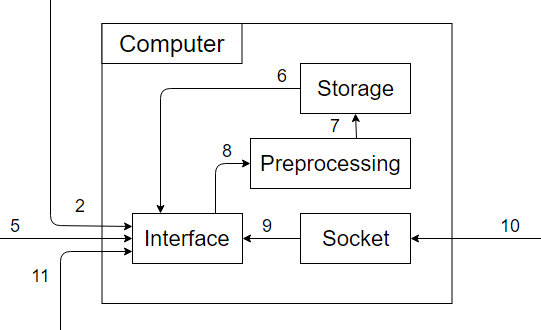
\includegraphics[width=0.60\textwidth]{images/computer_subsystem.png}
 \caption{Socket subsystem diagram}
\end{figure}

\subsubsection{Assumptions}
Assume the electrical socket will not malfunction and correctly sends the desired electrical power for the Traffic Pi to correctly work.

\subsubsection{Responsibilities}
The socket sub-layer will transfer the desired electrical power to the computer layer's interface and to maintain a steady electrical flow of power so the Traffic Pi can continue to function. The socket is depended on correctly receiving the required power from the power layer.

\subsubsection{Subsystem Interfaces}

\begin {table}[H]
\caption {Socket subsystem interfaces} 
\begin{center}
    \begin{tabular}{ | p{1cm} | p{6cm} | p{3cm} | p{3cm} |}
    \hline
    ID & Description & Inputs & Outputs \\ \hline
    \#9 & Mechanical socket transmitting electrical power & \pbox{3cm}{N/A} & \pbox{3cm}{Electric power (watts)}  \\ \hline
    \#10 & The physical implementation of an electric flow of power that allows the device to function & \pbox{3cm}{Electric power (watts)} & \pbox{3cm}{N/A}  \\ \hline
    \end{tabular}
\end{center}
\end{table}

